%%%%%%%%%%%%%%%%%%%%%%%%%%%%%%%%%%%%%%%%%%%%%%%%%%%%%%%%%%%%%%%%%%%%%%%%%%%%%%%
\chapter{基于依赖链与检索增强生成的代码变更影响分析}

\section{引言}

% 在软件系统的开发周期中,随着整体架构的日益复杂以及规模逐渐扩大,程序员在进行功能迭代、Bug修复等任务时,往往会面临较大的挑战。尤其是在庞大的代码库中,程序员难以快速且高效地评估某一变更对整体系统的影响。因此,若能在工作中引入一种高效的系统或算法来自动化地分析代码变更所带来的潜在影响,将极大地提升程序维护人员的工作效率。这不仅有助于减少潜在漏洞的发生,也能够确保系统在不断演进的过程中保持高质量和稳定性。由此可见,代码变更影响分析成为了软件开发中一个亟待关注的关键问题,值得深入研究与探讨。

由于代码预训练模型优秀的泛化能力和知识迁移能力,第二章中基于代码预训练模型的变更影响分析方法相较于基于方法间关系的方法具有更优秀的性能。但是由于其计算效率问题,导致其在实际使用时较为耗时。除此之外,由于该方法仅靠两两方法的代码进行变更影响关系的检测,因此方法代码中无法反映的间接依赖信息在检测时缺失了,导致其在间接依赖的影响关系判断上表现不好。

检索增强生成(Retrieval Augmented Generation,RAG)技术由Lewis 等人\cite{2020Retrieval}于 2020 年提出,是一种将信息检索与生成式模型(如 GPT 等)相结合的技术,它可以在文本生成过程中有效利用外部知识库或数据库中的信息,以提高生成结果的准确性和上下文相关性。RAG工作流程可以概括为两步,检索和生成。检索过程中根据输入查询(query),从外部知识库(如文档库、网页、数据库)中检索与输入相关的上下文或片段,生成阶段将检索到的信息与用户的输入结合起来,作为生成模型的输入,生成模型根据检索的上下文生成答案或内容。RAG方法能有效解决端到端问答模型的效率问题和减少事实错误的发生。

为了进一步提升代码变更影响分析的效率和可用性,本章提出了一种基于依赖链与检索增强生成的代码变更影响分析算法。本方法以代码库中的海量方法为知识库,通过信息检索技术,生成候选方法集合,如果候选方法中有与变更方法存在间接依赖关系的方法,则根据代码依赖图提取调用路径上的中间方法,构造推理信息。利用当前大规模语言模型在各种文本领域上强大的语义理解和生成能力,准确的判断候选集合中的变更影响关系。

% 在该算法中,信息检索模块能够显著降低计算时间,确保在大规模代码库中快速定位相关代码,通过提供调用路径的中间方法,保证模型判断时的代码逻辑的完整性,而大语言模型部分则保证了变更影响关系分析结果的高准确性。此外,通过动态调整候选集合的大小,可以有效平衡算法的运行速度与分析效果,从而使得整个系统既高效又可靠,能够在实践中为程序维护和优化提供有力支持。

\section{研究动机}

上一章节所提出的基于代码预训练模型的变更影响分析方法,尽管在测试基准方面取得了当前最优的效果,然而,其仍然存在两个较为显著的问题,即计算效率问题和间接依赖的语义缺失问题。

\textbf{计算效率问题:}每当需要针对代码库中的一个变更点展开变更影响分析时,都必须将变更方法与整个代码库的其他方法组对,然后输入模型进行检测。对于规模较大的项目代码而言,这种方法所带来的计算延迟会严重影响其可用性,几乎使其无法正常使用。

针对该问题,可以考虑将对方法的编码与变更关系的分析两个阶段进行解耦。在初始化阶段,运用嵌入模型对代码库的全部方法进行编码并存储。当需要对某个变更点进行分析时,仅需通过向量相似度计算筛选出少量候选方法,利用大语言模型优越的语义理解能力进行其变更影响关系的判断。

\textbf{间接依赖的语义缺失问题:}由于基于代码预训练模型的算法仅依据两个方法的代码来判断变更影响关系,因此当两个方法之间存在间接依赖时,如果不提供中间方法的调用逻辑,相关信息便会缺失,这将导致模型无法合理推断方法之间的变更影响关系。在这种情况下,只有资深工程师凭借对方法功能的了解,结合丰富的经验才能够完成判断,但即便如此,也很难保证判断的正确性。

\begin{figure}[htbp]
\centering
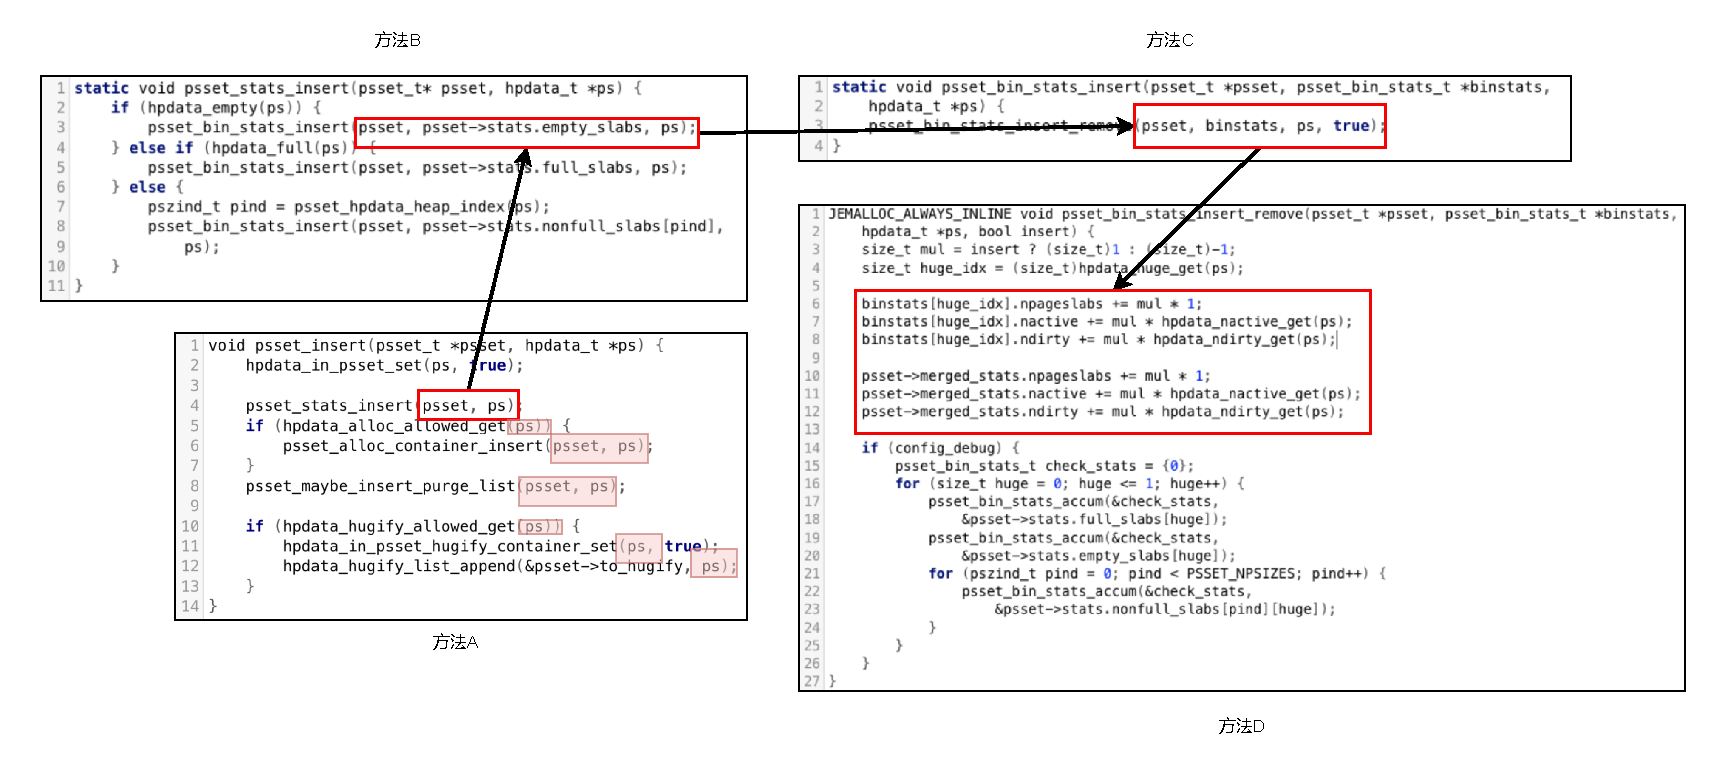
\includegraphics[width = 1\textwidth]{figures/3_间接依赖例子.pdf}
\caption{方法间间接依赖型变更影响关系实例}
\label{3_间接依赖例子}
\end{figure}

这里以jemalloc项目中的一对有变更影响关系的方法为例,说明这类间接依赖型关系的出现原因和判断难度。如图\ref{3_间接依赖例子}所示,该例中共包含4个方法,分别是psset\_insert、psset\_stats\_insert、psset\_bin\_stats\_insert和psset\_bin\_stats\_insert\_remove,后文简称为方法A、B、C、D。它们的调用关系为A $\rightarrow$ B $\rightarrow$ C$\rightarrow$ D。其中方法D与方法A之间存在变更影响,这是由于在方法A中向下游方法传递了变量psset和ps,在方法B和C中,均未对这两个变量进行操作,而是继续向下游传递。而在方法D中,直接对这两个变量进行了更改,由于这两个变量是指针类型,因此更改直接反映在了对应的内存变量上,而在方法A调用返回后的代码逻辑中,存在6处直接使用了这两个更改后的变量,一旦这两个变量的操作逻辑在方法D中有所改变,那么将会间接影响到方法A中对该变量的访问、操作逻辑,因此方法A和方法D之间存在由间接依赖导致的变更影响关系,主要表现在数据流传递过程中的变更-访问操作。而方法B和C与方法D之间则不存在变更影响关系,原因就在于其并未访问变更后的变量,只是进行了简单的数据传递。值得注意的是,如果仅依靠方法A和方法D的方法体,这样的依赖信息是丢失的,尤其是在数据传递的过程中,变量并不一定保持原来的名称,如在方法B中到方法C的传递中,将变量psset$\rightarrow$stats.empty\_slabs转化为了以变量名binstats标识的变量,判断难度进一步加大。




针对该问题,可以考虑在判断间接依赖的方法之间的变更影响关系时,提供其调用路径中的中间方法,补全缺失信息,以便为模型提供支持,实现准确的判断。

因此,本章提出了基于依赖链与检索增强生成的代码变更影响分析技术。该技术借助检索方式和代码依赖图,分别解决计算效率问题以及间接依赖所带来的语义缺失问题,从而提升变更影响分析在实际应用中的效果。

\section{整体流程设计}

为了解决第二章中基于代码预训练模型方法的计算效率问题与间接依赖语义缺失问题,本章提出了基于依赖链与检索增强生成的变更影响分析方法。图\ref{2_基于代码依赖与检索增强生成的变更影响分析方法框架}中展示了本章方法的研究框架。本章的方法主要流程分为三个模块:

\begin{enumerate}

    \item 数据构建模块。主要构建两个部分的数据:(1)依赖关系图。构建项目代码对应的依赖关系图,以支持后续间接调用的检测与查询。(2)原始知识库。将项目代码按方法的粒度进行提取,得到以方法为单元的集合作为原始知识库。(3)嵌入模型训练需要的三元组语料。将完整代码库按照方法的粒度进行切分并作为知识库。以上一章节的依赖闭包、克隆检测、共现关系挖掘三种方法检测出的变更影响关系为原始数据,基于大语言模型与代码依赖图进行数据清洗,构建准确的变更影响关系方法三元组(查询,正例,负例),用于训练嵌入模型,使嵌入模型专精于检测变更影响关系这一垂直领域。

    \item 检索模块。在三元组语料上训练嵌入模型,训练后使用嵌入模型对知识库进行预编码。在测试时仅需对查询方法进行编码,并与知识库中的向量计算相似度,找出相似度最高的前$k$个(top-$k$)作为候选方法。
    
    \item 增强生成模块。构建由查询方法,候选方法集合,调用路径的中间方法(如有)组合成的提示,使用大语言模型对候选方法进行判断,得到最终的有变更影响关系的方法。
    
\end{enumerate}

\begin{figure}[htbp]
\centering
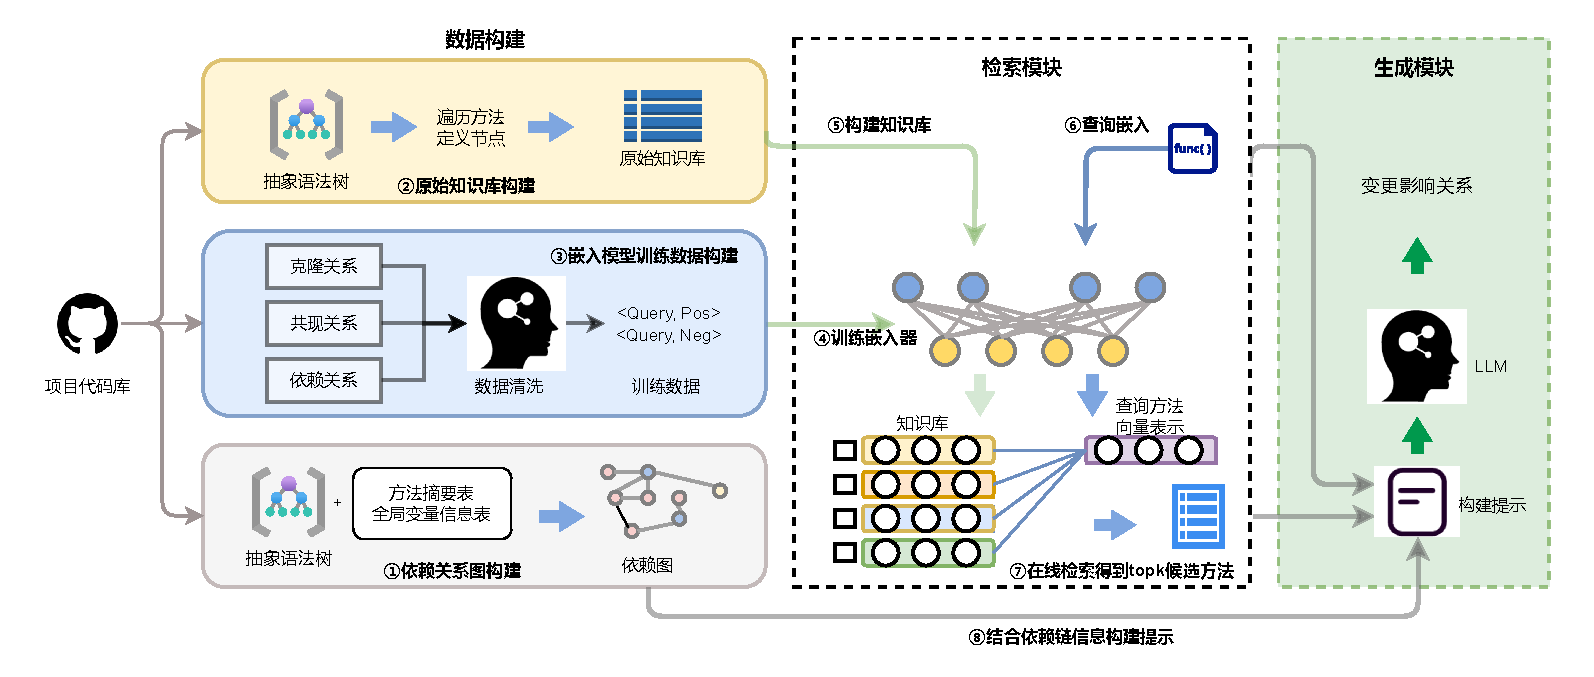
\includegraphics[width = 1\textwidth]{figures/3_第三章框架.pdf}
\caption{基于依赖链与检索增强生成的变更影响分析方法框架}
\label{2_基于代码依赖与检索增强生成的变更影响分析方法框架}
\end{figure}


\section{基于中间代码表示和关系挖掘方法的数据构建}
\label{3_数据构建}

数据构建主要分为三个部分,分别是依赖关系图构建、原始知识库构建以及嵌入模型训练数据构建。接下来进一步对这三部分数据构建进行介绍。

\noindent \textbf{1. 依赖关系图构建}

为在数据清洗过程和生成模块的推理过程中补充对依赖型变更影响关系的间接依赖信息,根据章节\ref{1_代码依赖图}所述步骤,基于抽象语法树、全局变量信息表和方法摘要表,构建以方法和全局变量为节点,以方法间的调用关系和方法对全局变量的引用关系为边的依赖关系图。

\noindent \textbf{2. 原始知识库构建}

为了将代码以更结构化和可管理的形式存储,便于后续进行嵌入和检索,需要对软件项目代码库进行分块。本方法检索的对象是方法,因此将软件代码按照方法进行分块最为合适。通过第二章中提到的代码预处理得到的抽象语法树,遍历其方法定义节点,得到每个方法的方法体,将方法体的集合作为知识库。

\noindent \textbf{3. 嵌入模型训练数据构建}

为了使嵌入模型专精于检测变更影响关系这一垂直领域,需要对嵌入模型进行训练,使具有变更影响关系的方法在向量空间中更接近,从而检索效果更好。因此需要构建训练嵌入模型所需的训练数据。

这里同第二章中基于代码预训练模型的方法类似,以基于依赖关系、克隆检测、共现关系挖掘三种方法检测出的变更影响关系为原始数据,假设得到的变更影响关系对集合为$S_{raw}$,其中$<Code_i,Code_j>\in S_{raw}$。参考上一章节的实验部分可知,$S_{raw}$中存在部分误报关系,如果不加处理,会严重影响检索模块的准确性。因此本文使用大语言模型对收集的数据进一步清洗,以得到足够准确的正例对。

值得注意的是,第二章中在对数据集进行清洗时仅提示了两个方法的具体信息,对于存在间接依赖方法的中间调用信息有所缺失,才导致其对于间接依赖导致的变更影响关系检测效果较差。因此在这一章中我们考虑结合依赖路径进行数据清洗。对于每一对方法$<Code_i,Code_j>$,数据清洗的具体流程如下:


(1)判断依赖可达性。根据代码依赖图判断两个方法之间是否存在调用关系,如果是直接调用,则无需处理。如果是间接调用,则需要补充调用路径的中间方法为$<Code_i,Code_{mid_1},Code_{mid_2},Code_j>$。

(2)基于大语言模型进行变更影响关系判断。利用代码语义和语言理解能力均较为出色的大语言模型,为原始数据$S_{raw}$中的每一组数据构建如图\ref{2_数据清洗prompt}的提示,进行变更影响关系的判断,剔除大模型认为没有变更影响关系的数据,剩下的数据整合为$S_{filtrate}$,其中$<Code_i,Code_j>\in S_{filtrate}$。

\begin{figure}[htbp]
\centering
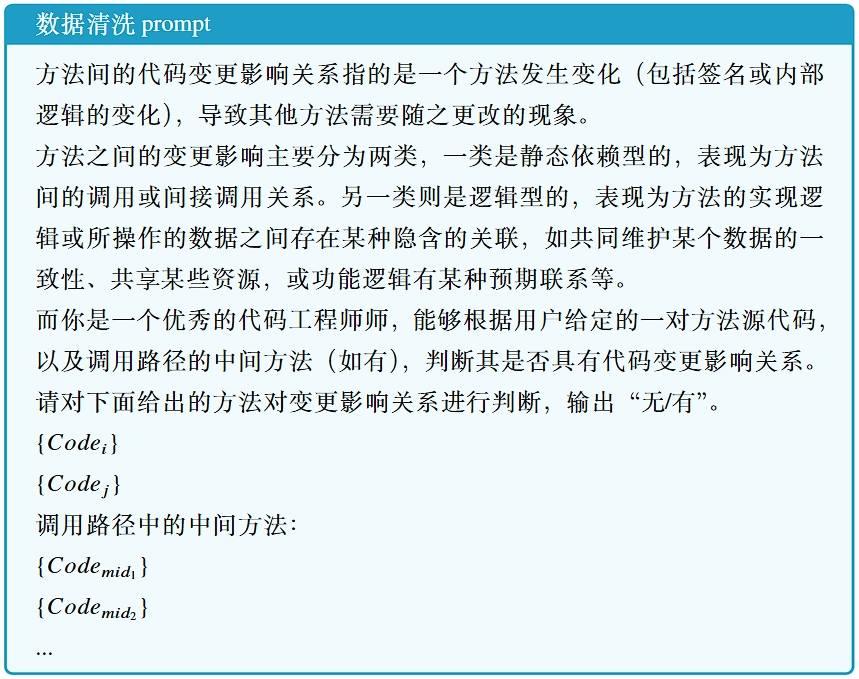
\includegraphics[width = 0.85\textwidth]{figures/2_数据清洗prompt.png}
\caption{数据清洗所使用的的Prompt}
\label{2_数据清洗prompt}
\end{figure}

为训练嵌入模型,还需构建正例所对应的负例,得到训练嵌入模型所需的$<Query,Pos,Neg>$三元组数据。对于每组正例数据数据$<Code_i,Code_j>$,随机挑选其中一个方法作为查询$Code_{query}$,另一方法作为正例$Code_{pos}$统计$S_{filtrate}$中出现的$Code_{query}$的正例集合 $\{Code_{pos},Code_k,Code_e,Code_k,\}$,从代码库中除正例集合之外的方法中随机采样方法作为负例$Code_{neg}$,将构建好的三元组数据$<Code_{query},Code_{pos},Code_{neg}>\in S$作为嵌入模型的训练数据,之后简写为$<Query,Pos,Neg>$。




\section{基于语义向量的变更影响候选方法检索}

检索模块主要分为离线和在线两个阶段,离线阶段涉及到嵌入模型训练与向量化知识库构建,在线阶段则涉及到嵌入检索与候选生成。接下来详细介绍两个阶段的主要任务和关键步骤。

\subsection{嵌入模型训练与向量化知识库构建}


离线阶段的主要任务是完成嵌入模型的训练,并对知识库中每个方法进行嵌入。具体而言,嵌入模型通过对代码库中的每个方法进行编码,将其转换为具有语义信息的稠密向量表示。这些嵌入向量随后被存储在知识库中,为后续的检索任务提供数据基础。

\noindent \textbf{1.嵌入模型训练}

本文中嵌入模型用于将方法代码这种长度不一、非对齐的形式转换为固定长度的稠密向量表示,即将方法的token序列$code={t_1, t_2, ..., t_n}$转化为对应的向量表示$E_code$。

向量检索的原理是将查询向量与知识库中的向量计算相似度,返回向量相似度最高的若干条作为候选向量。因此相似度计算的准确性尤为重要。在检测方法间变更影响关系的场景下,相似度越高则证明方法之间越容易存在变更影响关系,即这两个方法对应的向量在向量空间中有着更近的距离,而没有变更影响关系的方法对在向量空间中的距离则更远。

因此在训练嵌入模型时,对于训练数据中的三元组数据的嵌入$<E_{Query},E_{Pos},E_{Neg}>$,训练目标是将$E_{Query}$与$E_{Pos}$的相似度尽可能地提高,将$E_{Query}$与$E_{Neg}$的相似度尽可能地降低。本文选择对比损失函数(Contrastive Loss)中InfoNCE Loss(Noise Contrastive Estimation Loss)作为嵌入模型的损失函数进行训练。其定义为式\ref{2_损失函数}所示。InfoNCE Loss是一种用于自监督学习的损失函数,通常用于学习特征表示或者表征学习。它基于信息论的思想,通过对比正样本和负样本的相似性来学习模型参数。

\begin{equation}
    L_{InfoNCE} = -\log\frac{\exp(sim(E_{Query}, E_{Pos}) / \tau)}{\exp(sim(E_{Query}, E_{Pos}) / \tau)+\exp(sim(E_{Query}, E_{Neg}) / \tau)}
    \label{2_损失函数}
\end{equation}


其中,$\tau$为温度因子,用于控制相似度的平滑程度。$sim(E_{Query}, E_{Pos/Neg})$为查询向量和其对应的正例或负例样本的相似度,在相似度度量上本文选择余弦相似度进行计算,其定义如式\ref{2_相似度函数}所示。

\begin{align}
sim(A,B)&=\frac{A\cdot B}{\vert A\vert\vert B\vert}=\frac{\sum_{i = 1}^{n}x_iy_i}{\sqrt{\sum_{i = 1}^{n}x_i^2}\sqrt{\sum_{i = 1}^{n}y_i^2}} \\
A &= (x_1, x_2, \dots, x_n) \\
B &= (y_1, y_2, \dots, y_n)
\label{2_相似度函数}
\end{align}

其中A和B分别表示方法对的token序列编码后的向量表示。通过最小化$L_{InfoNCE}$来优化嵌入模型,从而提升查询向量与正样本之间的相似度,同时减少与负样本之间的相似度,使嵌入模型专精于变更影响关系这一任务。

\noindent \textbf{2.知识库构建}

在训练得到嵌入模型后,为了提高推理效率,需要将原始知识库中的方法通过嵌入模型转换为向量表示,从而构建编码后的知识库。该过程的目的是将每个方法转化为包含语义信息的稠密向量,以便在推理过程中实现高效检索。具体而言,利用前文中训练得到的嵌入模型对代码库中的每个方法 $Code_i$ 进行编码,得到其对应的向量表示 $E_{Code_i} = \text{Embedding\_model}(Code_i)$,其中 $E_{Code_i}$ 是一个包含该方法语义信息的稠密向量。编码完成后,所有方法的向量集合表示为 $\mathbf{E} = \{ E_{code_1}, E_{code_2}, ..., E_{code_n} \}$,其中 $n$ 是代码库中方法的总数,$\mathbf{E}$即为项目代码对应的知识库。


为了提高知识库检索的效率,本文采用FAISS(Facebook AI Similarity Search)作为稠密向量的检索工具。FAISS是一种高效的向量检索框架,能够对大规模向量数据进行索引并支持快速检索。通过构建向量索引,FAISS能够显著提高在大规模数据库中进行相似度搜索的速度。FAISS支持多种类型的索引结构,包括平坦索引、倒排文件索引和层次化导航图等,这些索引结构能够根据数据的规模、向量维度及存储需求,灵活应对不同查询速度和精度的需求。

鉴于本文的研究对象是软件项目代码,且分析粒度为方法级别,代码库中的方法数量通常较少,最多只有几千个方法。与处理文档类问答生成任务中涉及的大规模数据集不同,本文的代码库规模相对较小。因此,在构建索引时,本文选择了较为简单的平坦索引结构对方法向量进行检索。

\subsection{查询嵌入与候选检索}

在线阶段主要负责对每个新的查询进行实时处理,该阶段涉及两个关键步骤,旨在为查询方法检索候选的有变更影响关系的方法。以下是对该阶段的详细阐述:

\noindent \textbf{1.查询嵌入}

对于新的方法查询 $Query$,使用经过训练的嵌入模型对其进行嵌入操作,将方法转换为可与知识库中存储的向量进行相似度比较的形式。具体来说,通过将 $Query$ 输入到嵌入模型中,得到其对应的嵌入表示,即 $E_{Query}=Embedding\_model(Query)$。此嵌入表示 $E_{Query}$ 是一个稠密向量,它包含了查询的语义信息,能够有效地表示该查询在高维空间中的位置,为后续的相似度计算和检索过程奠定基础。在这一过程中,嵌入模型发挥着至关重要的作用,它依据自身在训练阶段所学习到的模式和特征,将具有不同语义特征的查询转化为具有独特特征的向量,从而确保在后续的检索和分析中能够准确地找到候选方法。

\noindent \textbf{2.在线检索}

在获得查询的嵌入表示$E_{Query}$之后,利用FAISS对知识库中的向量进行检索,由于FAISS不直接提供基于余弦相似度的检索方式,根据余弦相似度公式,可以结合其提供的基于点积的的检索方式和L2范数来达成基于余弦相似度的检索。选择与查询向量$E_{Query}$在余弦相似度上最为接近的$k$个向量。通过这些相似度最高的$k$个向量的索引,可以找到对应的源码方法,将其作为候选方法返回。

$top\ k$值的选择对检索结果的质量与效率有着直接影响。当$top\ k$值设置得较高时,检索模块能够召回更多的正确关系,因此查全率较高。然而,候选数量的增加会导致后续的大模型需要判断更多的候选方法,导致整个系统的处理速度可能会下降。相反,若$top\ k$值设置较低,则检索出的候选方法较少,查全率可能会较低,但大模型的计算效率会相对较高。因此,$top\ k$的选择需要根据实际使用场景的需求以及模型的能力进行权衡,以达到查全率与计算效率之间的最佳平衡。

\section{基于依赖链与大语言模型推理的生成方法}

生成模块旨在利用大语言模型出色的自然语言和代码语义理解能力,分析查询方法 $Code_{query}$ 与检索出来的候选方法集合 $\{Code_1, Code_2, ..., Code_k\}$ 之间的代码变更影响关系。在进行变更影响判断之前,需要首先通过代码依赖图来判断查询方法与候选方法之间是否存在调用关系,如果是直接调用或逻辑型的依赖,则无需处理。如果是间接调用,则需要补充该调用路径中的中间方法,以形成完整的调用链,如$<Code_{query},Code_{1_{mid_1}},...,Code_{1_{mid_2}},Code_1>$。

为根据查询和依赖分析的结果动态构建推理提示,通过槽位填充的方式进行构建,如图\label{2_推理prompt}所示。值得注意的是,为了包含依赖路径关系,这里候选方法是以组的形式出现的,如果组内元素个数不为 1,则说明该组的主要候选方法是与查询方法存在间接调用关系的方法,则提示对应的路径信息,否则直接进行推理。填充的方式如图所示。[x] 表示查询方法,[z] 表示检索到的候选方法,存在间接依赖的方法则对路径信息进行补充,构造得到对应的提示。

\begin{figure}[htbp]
\centering
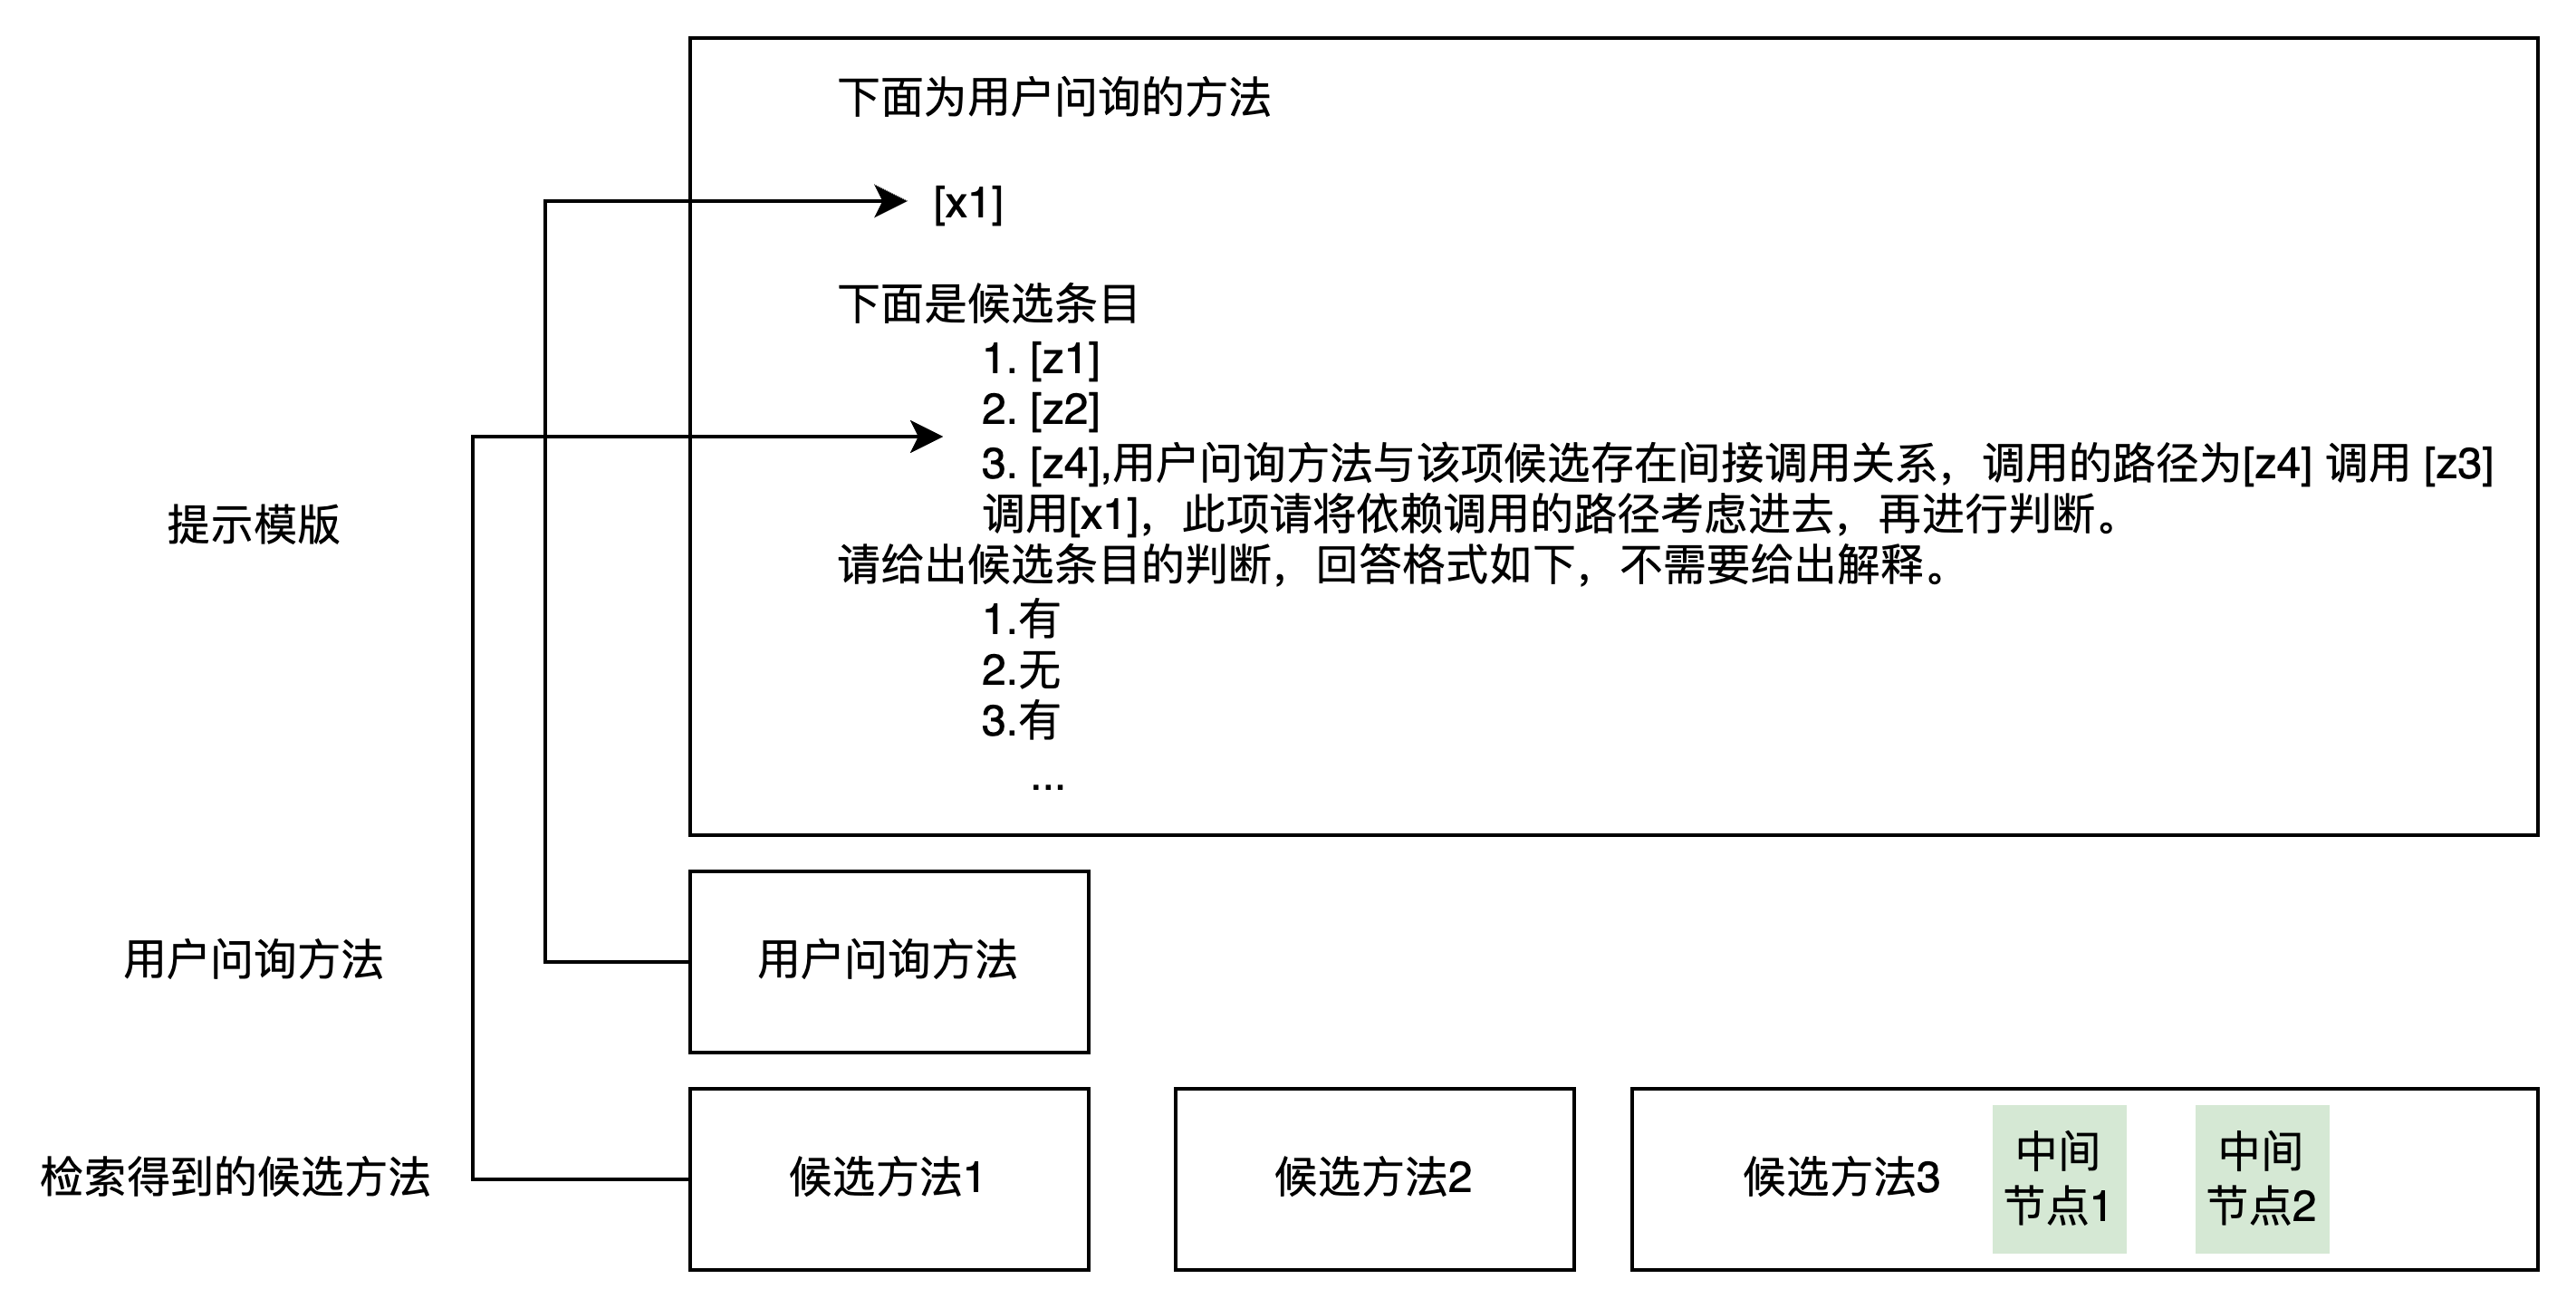
\includegraphics[width = 0.9\textwidth]{figures/提示词填充.jpg}
\caption{动态构建生成模块所使用的提示}
\label{2_推理prompt}
\end{figure}


将大语言模型的回复进行解析即可得到与查询方法有变更影响分析的方法。对于有$N$个方法的项目,在实际使用时对于每个查询,需要进行$N$次相似度计算,调用$1$次大模型进行推理,如果上下文长度过长可以对候选方法分片,多次调用大模型,相比于基于代码预训练模型的方法每次需要$N$次的模型前向计算,不仅节省了大量计算时间,还提升了系统的查全率和查准率,在实际应用场景中是更好的选择。


\section{实验结果与分析}

\subsection{实验数据}

为了便于与前文方法进行性能对比,本章的测试数据与第二章相同,具体信息见表\ref{1_test_data_info}所示。

对于嵌入模型所需的三元组训练数据,本章中数据清洗的方法新增了对依赖路径信息的补充,数据集的收集过程如\ref{3_数据构建}节中所述。在数据清洗过程中,所使用的模型为Doubao(API模型名:Doubao-lite-32k-240428)。最终得到的训练数据的统计信息如表\ref{1_数据集统计信息}所示,共计包含4289对数据。这些数据将用于嵌入模型的训练。


\begin{table}[htbp]
\caption{嵌入模型训练数据统计信息}
\label{1_数据集统计信息}
\vspace{0.5em}\centering\wuhao
\begin{tabular}{cccc}
\toprule
项目名称 & 三元组数量 \\
\midrule
TheAlgorithms    & 314   \\
antiword-0.37    & 257   \\
jemalloc-5.3.0   & 1023   \\
libbpf-1.1       & 835   \\
librdkafka-2.1.0 & 1524  \\
FFmpegKit-5.1.0  & 336   \\ 
总计              & 4289  \\
\bottomrule
\end{tabular}
\end{table}

\subsection{评价指标} 

评价指标与第\ref{1_评价指标}节一致,采用Precision(精确率)、Recall(召回率)和F-measure来全面评估模型在检测变更影响关系中的表现。这些指标可以有效衡量模型在实际应用中的能力,

\subsection{实验设置}

\noindent \textbf{1. 检索模块嵌入模型选择}

MTEB Leaderboard\footnote{https://huggingface.co/spaces/mteb/leaderboard} 是一个实时更新的开源嵌入模型排行榜,专门用于评估不同模型在各种任务中的嵌入能力。为了实现对原始知识库中方法代码的有效编码,本文从MTEB Leaderboard中选取适合本任务的嵌入模型。选择标准主要包括以下几点:(1)模型在开源嵌入能力评价基准上表现优异,这能够体现其在各类通用文本上的嵌入能力。(2)模型支持的上下文长度大于4k,考虑到代码任务通常涉及较长的上下文,较短的上下文长度可能无法有效捕捉到代码间的复杂关系。(3)模型的参数规模控制在500M以下,综合考虑计算资源和数据规模,超过500M参数规模的模型在使用上的代价较高,难以满足实际应用需求。基于这些选择标准,本文最终选定了如表\ref{2_嵌入模型参数量}所示的5个模型。这些模型在性能、上下文支持以及资源消耗方面都达到了较好的平衡,适合本文中对代码片段进行嵌入编码的需求。
    
    \begin{table}[htbp]
    \caption{嵌入模型信息}
    \label{2_嵌入模型参数量}
    \vspace{0.5em}\centering\wuhao
    \begin{tabular}{ccc}
    \toprule
    嵌入模型 & 参数量 & 上下文长度  \\
    \midrule
    gte-large-en-v1.5 & 434M & 8192 \\
    jina-embeddings-v3 & 572M & 8192\\
    stella\_en\_400M\_v5 & 435M & 8192 \\
    KaLM-embedding-multilingual-mini-instruct-v1.5 & 494M & 131072 \\
    nomic-embed-text-v1.5 & 137M & 8192 \\
    \bottomrule
    \end{tabular}
    \end{table}

\noindent \textbf{2. 嵌入模型训练设置}

本文在嵌入模型的训练过程中,采用了对比损失函数InfoNCE Loss作为目标函数,以确保模型能够有效学习到不同代码片段之间的相似度关系。训练优化器选择了Adam优化器,其中超参数$\beta_1$设置为0.9,$\beta_2$设置为0.95。为提高训练效果,学习率采用余弦衰减策略,使得训练过程中学习率逐渐减小,有助于模型在接近收敛时获得更精细的更新。

Batch size固定为64,以保证每次梯度更新的稳定性。对于较大规模的模型,考虑到内存限制,采用了梯度累计(Gradient Accumulation)技术,通过多次反向传播累积梯度,从而保证了相同的批次大小。学习率初始值设置为1e-4。

所有实验均在PyTorch框架和Transformer库上实现,确保了高效的模型训练和易于扩展的实现平台。训练过程在单个NVIDIA Tesla V100 32G GPU上进行。

\noindent \textbf{3. 生成模型选择}
    
本章实验中生成模块使用的大模型包含两类,分别是闭源商业模型和开源模型。其中闭源模型包括:GPT-4o-mini(API model name:gpt-4o-mini-2024-07-18),Doubao(API model name:Doubao-lite-32k-240428),Kimi(API model name:moonshot-v1-32k)。开源模型选择:Qwen2.5-Coder-3B-Instruct ,Llama-3.2-3B-Instruct


\subsection{实验结果与对比分析}

RQ1:经过训练后的检索模块性能如何,与0样本嵌入模型相比是否更专注于变更影响关系检测?能否有效检索到与查询方法存在变更影响关系的方法?

RQ2:本章提出的基于依赖链与检索增强生成的变更影响关系分析方法性能如何,相比于其他方法,其在精确率,召回率和 F-measure上表现如何?

RQ3:本章提出的基于依赖链与检索增强生成的变更影响关系分析方法是否能有效解决间接依赖信息缺失的问题?

RQ4:本章提出的基于依赖链与检索增强生成的变更影响关系分析方法的跨项目迁移表现如何?
 

\textbf{1.针对于RQ1的实验}

本实验通过计算$topk$中k值与召回率的关系,验证检索模块嵌入模型的性能。实验结果如表\ref{1_检索模块的召回率与Topk的关系可视化}所示。其中横坐标表示$topk$值,即检索模块在知识库中检索到的相似度排序的前$k$个,纵坐标表示召回率。虚线为未经训练的嵌入模型,实线表示经过训练的嵌入模型。

\begin{figure}[htbp]
\centering
\includegraphics[width = 1\textwidth]{figures/topk召回率可视化.pdf}
\caption{检索模块的召回率与Topk关系}
\label{1_检索模块的召回率与Topk的关系可视化}
\end{figure}

经过分析可以发现,总的来讲,除模型KaLM-embedding-v1.5之外,经过训练的嵌入模型在本文应用场景的性能普遍优于未经训练的模型,其中模型KaLM-embedding-v1.5较为特殊,在0样本的情况下其本身性能差于其他模型,因此训练后虽有提升,但还是难以超越其他模型未经训练的版本。

对于未经训练的嵌入模型来讲,模型stella\_en\_400M\_v5表现最好,但在k最大为30的设置下也只能达到50\%左右的召回率,这说明对于查询方法来讲,有近一半的与其有变更影响关系的方法未被检索出来,性能一般。而经过训练的嵌入模型普遍优于未经训练的模型,其中stella\_en\_400M\_v5模型的综合表现最佳。在k为15到30的区间,召回率均高于其他模型,尤其在k为最高30时,能达到近90\%的召回率。因此可以得出结论,训练后的检索模块性能较强,与未经训练的模型相比,能更专注于检测变更影响关系的任务。

对于$topk$的k值,可以发现k值越大召回率越高,这是由于在召回率较小的时候,检索到的候选方法较少,甚至真实正例数即能超过该k值。而$topk$值越大,则检索到的包含真实正例的概率也越大,因此召回率越高。


考虑到训练后嵌入模型的性能和$topk$的k值大小对推理速度和召回率产生影响,综合考虑选择模型stella\_en\_400M\_v5作为嵌入模型,$topk=20$作为后续实验的设定。 

\textbf{2.针对于RQ2的实验}

实验结果如表\ref{2_不同LLM的实验表现}所示。总的来讲,基于大语言模型的方法的检测性能均优于基于代码预训练模型的方法,即使是最小的开源模型Qwen2.5-Coder-3B-Instruct ,Llama-3.2-3B-Instruct,其在F-measure、召回率和精确率的表现也可以超过经过上一章节训练的CodeBERTa模型。

\begin{table}[htbp]
\caption{不同LLM的实验表现}
\label{2_不同LLM的实验表现}
\vspace{0.5em}\centering\wuhao
\begin{tabular}{cccc}
\toprule
方法 & F-measure & recall & precision  \\
\midrule
CodeBERTa & 59.5 & 55.3 & 64.4 \\
Just Retrieval & 32.6 & \textbf{78.1} & 20.6 \\
\midrule
RAG-GPT4o & \textbf{75.8} & 74.6 & \textbf{77.1} \\
RAG-Doubao & 73.4 & 73.8 & 73.1 \\
RAG-Kimi & 70.2 & 71.2 & 69.2 \\
RAG-Qwen2.5 & 65.4 & 63.5 & 67.4 \\
RAG-Llama-3.2 & 64.9 & 62.3 & 67.8 \\
\bottomrule
\end{tabular}
\end{table}

为了更好地评估大语言模型在变更影响关系检测任务中的重要性,本实验进一步与仅使用检索模块的方案进行了对比分析。从实验结果可以看出,单独使用检索模块的方案在召回率上表现最佳,达到了引入生成模型后性能的上限。这一现象的原因在于,大语言模型只在检索到的候选结果基础上进行进一步判断,因此,它的作用是减少而非增加变更影响关系的检测结果。由于设定了$topk=20$,检索过程中不可避免地会出现误报,这导致了该方法的准确率相对较低。

然而,在加入生成模块之后,召回率略有下降,但精确度却提升了47.2\%至55.5\%,这充分证明了大语言模型在代码语义理解基础上判断变更影响关系的强大能力。通过结合检索模块和生成模块,RAG方法能够在提高查全率的同时,显著提升查准率,确保检测过程中的全面性和准确性。

此外,选择不同的大语言模型作为生成模块,其对检测任务的表现也存在一定差异。总体而言,闭源商业模型的性能优于开源模型。具体来说,以GPT4o为生成模块的RAG方法展现出了最佳的综合性能,其在召回率和准确率上均表现优异。而Doubao和Kimi模型的表现稍逊一筹,尽管在召回率上与GPT4o接近,但精确率存在明显差距,可能是由于这些模型对代码语义的理解能力相对较弱所致。而开源模型之间的表现相对平衡,尽管它们的整体效果略低于闭源商业模型,这可能与模型规模和架构设计存在差异有关,但相比于基于代码预训练模型的方法,仍然表现出了显著的优势。

综上所述,生成模块在变更影响关系检测中的作用不可忽视,它在变更影响分析任务中的体现出了强大的代码语义理解能力,能够有效提升检测的精确率。尽管闭源商业模型的表现更为优越,但开源模型依然提供了一个具有竞争力的选择,在实际应用中具备较好的实用价值。

\begin{table}[htbp]
\caption{变更影响实验结果}
\label{2_变更影响实验结果}
\vspace{0.5em}\centering\wuhao
\begin{tabular}{c|ccc|ccc|c}
\toprule
  & \multicolumn{3}{c|}{Dependence-Based} & \multicolumn{3}{c|}{Logic-Based} & Overall \\
\midrule
方法 & F-measure & recall & precision & F-measure & recall & precision  
 & F-measure\\
\midrule
依赖闭包 &  44.8 & 100 & 28.9 & - & - & - & 36.8 \\
克隆检测 &  - & - & - & 31.8 & 19.1 & 95.7 & 3.8\\
共现关系挖掘 &  56.0 & 44.6 & 75.4 & 57.0 & 47.3 & 71.8 & 52.8\\
CodeBERTa  &   61.9 & 56.6 & 68.3 & 71.7 & 73.9 & 69.7 &59.5\\
Just Retrieval   & 34.5 & 82.3 & 21.8 & 36.6 & 88.5 & 23.1 & 32.6\\
RAG & \textbf{79.8} & 78.4 & 81.2 & \textbf{86.9} & 85.9 & 87.9 & \textbf{75.8}\\
\bottomrule
\end{tabular}
\end{table}

为了进一步分析RAG方法与其他方法在不同类型的变更影响关系上的检测效果,本实验对比了不同方法在依赖型和逻辑型的表现,得到的结果如表\ref{2_变更影响实验结果}所示。对比可以发现相比于其他方法来讲,基于依赖链与检索增强生成的方法在两个类型的变更影响关系检测上,均拥有更好的性能。这表明,基于依赖链与检索增强生成的方法在处理依赖型和逻辑型变更影响关系时,具有更强的检测能力。

依赖型关系和逻辑型关系有着本质的差异,分别侧重于不同方面的代码间联系。而RAG方法在这两类关系的检测上均展现了优越的性能。依赖型影响关系的判定依赖于方法间的直接或间接调用。前文方法在处理间接依赖时存在信息缺失,而RAG方法通过结合代码依赖图和检索模块,能够定位到相关方法并补充缺失的调用路径,显著提高了依赖型关系的召回率和准确率。在这一任务中,F-measure的提升达到16.9\%,有效减少了漏报的情况。而逻辑型影响关系主要关注代码的逻辑层面,涉及程序控制结构和功能实现之间的复杂交互。在这类关系中,对代码的语义理解尤为重要,RAG方法通过引入大语言模型的语义理解能力,能够深入分析代码的结构和功能逻辑,精准地判断代码变更对系统的影响。逻辑型关系的F-measure提升达到15.2\%,表明RAG方法在这方面的优势同样显著。

总的来说,RAG方法通过结合检索模块和大语言模型的优势,在依赖型和逻辑型变更关系的检测中均取得了显著的性能提升。依赖型关系的检测通过更精准的依赖路径识别提高了查全率,而逻辑型关系的检测则通过对代码语义的深度理解提升了精确度。两者结合,使得RAG方法在变更影响分析任务中展现了更强的适应性和准确率。

\textbf{3.针对于RQ3的实验}

为了验证依赖路径在变更影响关系检测中的重要作用,并探讨将调用路径中的中间方法纳入提示对间接依赖检测效果的提升,本实验选择了测试集中的间接依赖型变更影响分析子集进行验证。为了深入分析其贡献,设计了依赖路径消融实验,结果如表\ref{2_消融实验}所示。

\begin{table}[htbp]
\caption{加入调用路径的中间方法对间接依赖的检测效果的影响}
\label{2_消融实验}
\vspace{0.5em}\centering\wuhao
\begin{tabular}{cccc }
\toprule
  & \multicolumn{3}{c}{Indirect-Dependence-Based}  \\
% \midrule
方法 & F-measure & recall & precision \\  
\midrule
CodeBERTa  &  10.7 & 15.1 & 8.3 \\
\midrule
RAG without 依赖路径  & 14.2 & 12.1 & 17.1 \\
RAG  & 72.6 & 73.5 & 71.7 \\
\bottomrule
\end{tabular}
\end{table}



分别与第二章方法和未加入依赖路径的RAG方法进行对比,根据结果可以看出在提示中加入路径的中间方法对于检测效果的提升非常显著。与第二章方法相比,F-measure、召回率和精确率分别增加了61.9\%、58.4\%和63.4\%,与未加入依赖路径的方法相比,分别增加了58.4\%、61.4\%和54.6\%,说明方法中间的调用信息对变更影响关系的判断非常重要,如果丢失,则模型无法捕捉方法之间的联系,增加调用链能够补全这部分信息。

与第二章中提出的方法和未加入依赖路径的RAG方法分别进行对比,实验结果表明,在提示中加入依赖路径中的中间方法对变更影响关系的检测效果有显著提升。具体而言,与第二章方法相比,F-measure、召回率和精确率分别提高了61.9\%、58.4\%和63.4\%;与未加入依赖路径的RAG方法相比,F-measure、召回率和精确率分别提高了58.4\%、61.4\%和54.6\%。这些结果表明,方法调用链中间信息的加入对于变更影响关系的判断至关重要。缺少这些中间调用信息时,模型往往无法正确捕捉方法之间的内在联系,从而影响检测精度。通过引入调用链中的中间方法,模型能够有效弥补这一缺失,补全变更影响分析中的关键依赖信息,显著提高检测效果。

这一实验结果进一步证明了在提示信息中加入依赖路径不仅增强了模型对间接依赖的感知能力,也有助于提升整体变更影响关系分析的准确性和实用性。

\textbf{4.针对于RQ4的实验}

为了验证基于RAG的方法在跨项目场景下的泛化能力和知识迁移能力,本章设计了类似第二章的跨项目实验。数据集划分同上一章节一样,将项目分为四个分布内项目和两个分布外项目。在跨项目的实验设置下,模型仅在分布内项目上进行训练,而在测试时则只使用分布外项目进行验证。

\begin{table}[htbp]
\caption{跨项目迁移能力分析(F-measure)}
\label{2_跨项目迁移能力分析}
\vspace{0.5em}\centering\wuhao
\begin{tabular}{c|cccc|cc}
\toprule
方法& TheAlgorithms & antiword & librdkafka & FFmpegKit & jemalloc & libbpf\\
\midrule
train on 6 datasets & train &train &train &train &train &train \\
\midrule
CodeBERTa  &  60.23 & 59.64 & 60.18 & 57.87 & 60.99 & 58.22 \\
Just Retrieval   & 32.4 & 32.91 & 31.81 & 36.57 & 33.78 & 35.07  \\
RAG & 76.0 & 78.45 & 76.46 & 77.66 & 79.04 & 76.29  \\
\midrule
train on 4 datasets & train &train &train &train &test &test\\
\midrule
CodeBERTa  &  62.28 & 65.24 & 63.45 & 62.19 & 41.92$^*$ & 40.8$^*$\\
Just Retrieval   & 33.33 & 34.2 & 34.77 & 36.89 & 29.74$^*$ & 31.09$^*$ \\
RAG & 78.24 & 79.21 & 78.59 & 77.98 & 71.08$^*$ & 69.66$^*$ \\
\bottomrule
\end{tabular}
\end{table}

实验结果如表\ref{2_跨项目迁移能力分析}所示。通过对比分析,上一章节基于代码预训练模型的方法在跨项目测试时,性能下降幅度在28.9\%到31.7\%之间,显示出较为明显的性能衰减。而本章所提出的基于依赖路径和RAG的变更影响分析方法,在跨项目测试时性能下降幅度仅为9.2\%到11.4\%,显著低于基于代码预训练模型的方法。

这一结果表明,RAG方法在跨项目迁移时的性能下降较小,体现出更强的泛化能力,能够有效地将从一个项目中学到的变更影响模式迁移到新项目中,即使新项目的特征与源项目存在差异,系统依然能够维持较高的检测精度。这一优势不仅使得本章方法更贴近实际应用中的跨项目场景,也为变更影响分析提供了更广泛的适用性。相比之下,基于代码预训练模型的方法在面对不同项目时的表现较为不稳定,难以有效迁移学习到的模式,导致跨项目应用时性能明显下降。



因此,本章提出的基于依赖路径和RAG的变更影响分析方法不仅表现出较高的准确性,在跨项目中的泛化能力同样优秀,充分证明了该方法在多样化应用场景下的可行性和实用性。
 

\section{本章小结}

本章提出了基于依赖链与检索增强生成的代码变更影响分析方法,通过结合依赖路径提升了方法在间接依赖影响上的检测性能,并通过训练检索模块,大幅提升了测试集上的召回率,最后整个系统的综合表现得到了大幅提升。并且通过实验验证了依赖路径加入的有效性。最后在跨项目迁移能力的实验中,基于依赖链与检索增强生成的代码变更影响分析方法的迁移能力表现优秀,进一步证明了本章所提出的方法的有效性。

%%%%%%%%%%%%%%%%%%%%%%%%%%%%%%%%%%%%%%%%%%%%%%%%%%%%%%%%%%%%%%%%%%%%%%%%%%%%%%%